
%----------------------------------------------------------------------------------------
%	Lecture 21
%----------------------------------------------------------------------------------------

\chapter{Triple Integrals in Rectangular and Cylindrical Coordinates}

\bigbreak

\section{Triple Integrals}

Given a function $f(x, y, z)$ over some solid region of space $R$
then 
$$
\iiint f(x, y, z) dV = \iiint f(x, y, z) dx dy dz
$$
Here, $dV$ is the volume element which in Cartesian Coordinates becomes $dx dy dz$

{\bf Example 1. } Let's say our region is the region between two paraboloids : $z = x^2 + y^2$ and $z = 4 - x^2 - y^2$.
And we want to find the volume of the region so $$ Volume = \iiint 1 dV $$

\begin{figure}[ht!]
    \centering
    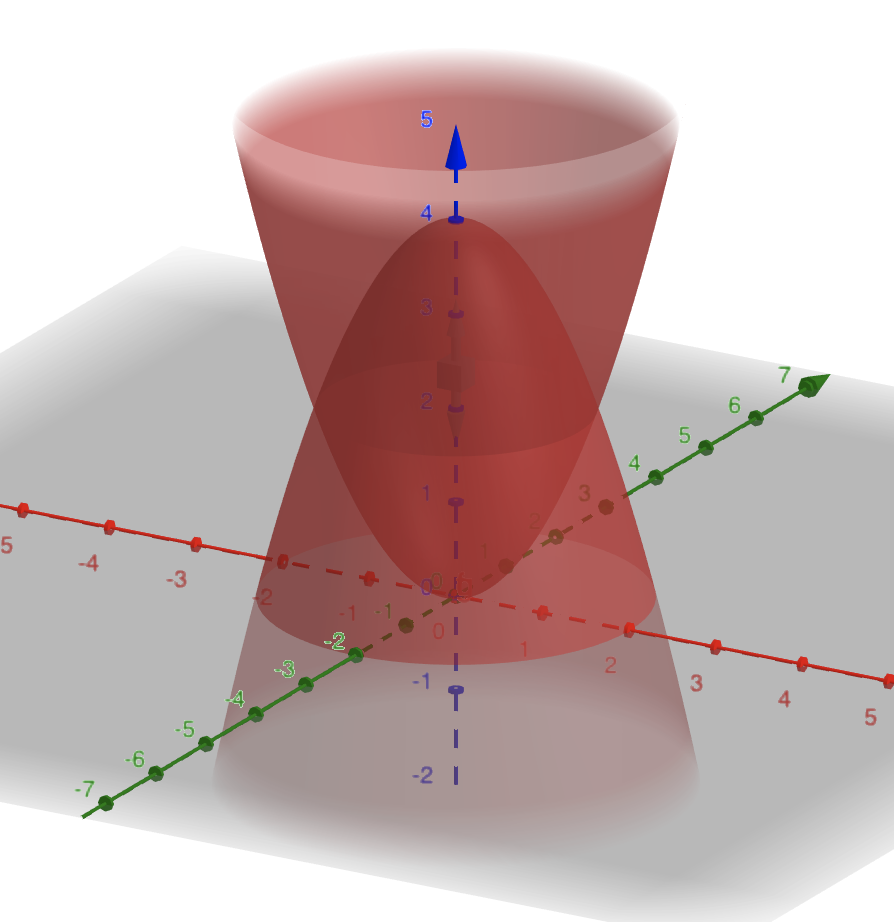
\includegraphics[scale=0.3]{./images/lecture_21_figure_1.png}
    \caption{Graph of the given region}
\end{figure}

We can see that the intersetion of these paraboloids will be a circle such that $x^2 + y^2 = 4 - x^2 + y^2 \Rightarrow x^2 + y^2 = 2$ in the plain $z = 2$.

It seems that integrating over $z$ first will be easier as it is given as a function of $x$ and $y$. So our integral becomes,
\begin{align*}
    Volume & = \int \int \int_{x^2+y^2}^{4-x^2-y^2} dz dy dx \\
        & = \iint 4 - 2x^2 -2y^2 dy dx \\
\end{align*}

Here we have reduced our triple integral to a double integral. 
The only thing that remains is to find the region. 
Our region will be the projection of our space region to the XY-plane. 
So here it will be a circle of radius $\sqrt{2}$ centered at origin.


Another way to say it is that our region is all the points where the upper limit of $z$ is less than the lower limit of $z$, that is, $x^2 + y^2 \leq 4 - x^2 - y^2$.
Solving this we get, $x^2 + y^2 \leq 2$. Thus,

$$
Volume = \int_{-\sqrt{2}}^{\sqrt{2}} \int_{-\sqrt{2-x^2}}^{\sqrt{2-x^2}} (4 - 2x^2 - 2y^2) dy dx
$$

Here we can also use symmetry and switch to polar coordinates. So our integral will become,

$$
Volume = \int_0^{2\pi} \int_0^{\sqrt{2}} \int_{r^2}^{4-r^2} dz \cdot r dr d\theta
$$

This integral is lot easier to evaluate.

Using $(r, \theta, z)$ is called the Cylindrical Coordinates.


\section{Applications}

\begin{enumerate}
    \item Finding Volume of Solids
    \item Finding Mass of the Solids : \ilds{\iiint \rho(x, y, z) dV} where $\rho(x, y, z)$ is the density of solids.
    \item Average value of a function $f(x, y, z)$ over a region $R$ : $$ \frac{1}{Volume(R)} \iiint_R f(x, y, z) dV $$
    \item Weigted Average of a function : $$ \frac{1}{Mass(R)} \iiint_R f(x, y, z) dV $$ 
    \item Center of Mass : $(Average(x), Average(y), Average(z))$
    \item Moment of Intertia about an axis : $$ \iiint (\text{distance to the axis})^2 \rho(x, y, z) dV $$  
\end{enumerate}
